\chapter{Effiziente Implementierungen}

%%% section %%%
\section{Langzahlen}

In (asymmetrischer) Kryptographie benötigen wir ülicherweise Werte, die weit größer sind, als die native Wortlänge der zugrundeliegenden Hardware.
Die meisten Register haben eine Wortlänge von 64 bit. Typische Schlüssellängen, beispielsweise für RSA Verschlüsselung, sind heutzutage 1024 bis 4096 bits.

\paragraph{Wie können solche Zahlen dargestellt werden?}

Eine Auswahl an Möglichkeiten ist:

\begin{enumerate}
    \item Residuen-Repräsentation \index{Residuen-Repräsentation}
    \item Verwendung von Arrays in nativer Wortgröße \index{Arrays mit nativer Wortgröße}
    \item Verwendung von Arrays kleiner als die native Wortgröße \index{Arrays kleiner als die native Wortgröße}
\end{enumerate}

\paragraph{Wie kann eine effiziente Modulo Reduktion implementiert werden?}

Die Division großer Zahlen ist sehr teuer, deswegen wurden Methoden für eine Restbestimmung ohne direkte Division entwickelt:

\begin{enumerate}
    \item Barrett Reduktion \index{Barrett Reduktion}
    \item Montgomery Arithmetik \index{Montgomery Arithmetik}
\end{enumerate}

\paragraph{Wie kann effizient Exponentiation implementiert werden}

Bei Square \& Multiply ist die Berechnung schneller, je weniger Bits des Exponenten den Wert \verb|1| haben, siehe NAF \index{NAF} (Non-adjacent Form) \index{NAF}.

%%% subsection %%%
\subsection{Residuen-Repräsentation} \index{Residuen-Repräsentation}

Wir wählen $r$ verschiedene koprime (paarweise teilerfremde) Moduli $m_1, \ldots, m_r$ und eine beliebige Zahl $x$. Wir können eine Darstellung

\begin{equation}
    x = (x_1, \ldots, x_r)
\end{equation}

wählen, wobei $x_i = x \mod m_i$ für $i = 1, \ldots, r$. Der chinesische Restsatz garantiert uns hierbei, die Rekonstruierbarkeit von $x$.

\paragraph{Vorteile}
Welche Vorteile hat diese Darstellung?  

\begin{itemize}
    \item Die Moduli $m_i$ können in nativer Wortgröße des Systems gewählt werden, die repräsentierten Zahlen haben eine Größe bis zu $\prod_i m_i = m_1 \cdot 
    ldots m_r$.
    \item Die Rechnung ist parallelisierbat, es braucht keine carry-propagation 
    \item Die meisten Grundrechenarten sind sehr einfach, weil sie mit der Modulo-Operation verträglich sind. Für die Addition, Subtraktion und Multiplikation haben wir
        \begin{align*}
            x + y     &= (x_1, \ldots, x_r) + (y_1, \ldots, y_r)     \\
                      &= (x_1 + y_1 \mod m_1, \ldots, x_r + y_r \mod m_r) \\
            x - y     &= (x_1, \ldots, x_r) - (y_1, \ldots, y_r)     \\ 
                      &= (x_1 - y_1 \mod m_1, \ldots, x_r - y_r \mod m_r) \\
            x \cdot y &= (x_1, \ldots, x_r) \cdot (y_1, \ldots, y_r) \\ 
                      &= (x_1 \cdot y_1 \mod m_1, \ldots, x_r \cdot y_r \mod m_r) 
        \end{align*}
\end{itemize}

\paragraph{Nachteile}
Welche Nachteile hat die Darstellung?

\begin{itemize}
    \item Der Vergleich zweier Zahlen ist aufwendig
    \item Die Division zweier Zahlen ist aufwendig 
    \item Rückrechnung in die gewöhnliche Zahlendarstellung aufwändig (Lösen simultaner Kongruenzen)
    \item Überlauf bei arithmetischen Operationen nicht detektierbar
\end{itemize}

\paragraph{Beispiel}

Wir berechnen die Residuen-Repräsentation von $x = 1820$ bezüglich der $(m_1, m_2, m_3, m_4, m_5) = (3,5,7,11,13)$. Wir haben $m = \prod_i m_i = 15015$.

\begin{align*}
    x \mod m_1 = 2 \\
    x \mod m_2 = 0 \\
    x \mod m_3 = 0 \\
    x \mod m_4 = 5 \\
    x \mod m_5 = 0 \\
\end{align*}

Das heißt die Darstellung von $x$ bezüglich $m$ ist $(2,0,0,5,0)$.  

Für die Rückrechnung von $(2,0,0,5,0)$ auf $1820$ lösen wir:

\begin{align*}
    x \equiv 2 &\mod 3 \\
    x \equiv 0 &\mod 5 \\
    x \equiv 0 &\mod 7 \\
    x \equiv 5 &\mod 11 \\
    x \equiv 0 &\mod 13 \\
\end{align*}

Wir berechnen für $m_1$ und $m_4$, wo der Modulus ungleich 0 ist

\begin{align*}
    M_1 = m / m_1 &= 15015 / 3 = 5005 \\
    M_4 = m / m_4 &= 15015 / 11 = 1365.
\end{align*}

Dann berechnen wir die Inversen bzgl. der Moduln $m_i$, z.B. mittels erweitertem euklidischen Algorithmus:

\begin{align*}
    y_1 = M_1^{-1} \mod m_1 = 5005^{-1} \mod 3 = 1 \\
    y_4 = M_4^{-1} \mod m_4 = 1364^{-1} \mod 11 = 1
\end{align*}

Somit können wir mittels Residuen $a_i = x \mod m_i$ berechnen 

\begin{align*}
    x &= \left(\sum_i a_i \cdot y_i \cdot M_i \right) \mod m \\
      &= 2\cdot 1 \cdot 5005 + 5 \cdot 1 \cdot 1365 \mod 15015 \\ 
      &= 1820.
\end{align*}

%%% subsection %%%
\subsection{Arrays in nativer Größe}

Sei $W$ die native Wortgröße eines Prozessors und $x$ eine Zahl, deren Binärdarstellung $n$ bit benötigt. Dafür verwenden wir das Array $A$, das $t = \lceil n/W \rceil$ Integers enthält.

\begin{figure}[h]
    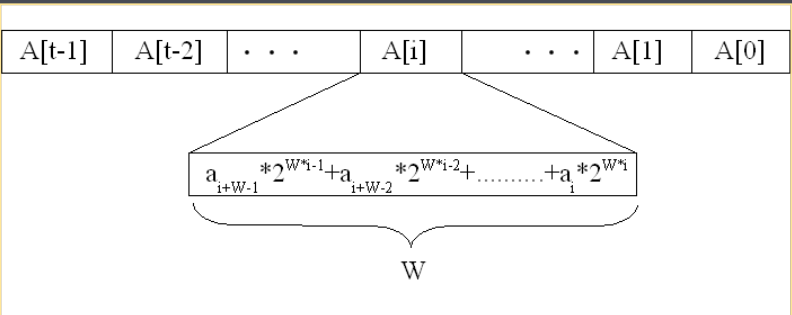
\includegraphics[width=0.8\textwidth]{figures/fig1-arrays-native-size}
    \centering
    \caption{Manuel Koschuch, Efficient Security for Mobile Communications Utilizing Elliptic Curves}
\end{figure}

\paragraph{Vorteile}

\begin{itemize}
    \item Die Langzahloperationen können auf Operationen auf nativer Wordgröße heruntergebrochen werden.
    \item Der zusätzliche Speicherbedarf ist maximal so groß wie ein natives Wort.
    \item Zugriff ist einfach und schnell.
    \item Vergleich von Langzahlen ist schnell und einfach.
    \item Verwendung von Langzahlen ist schnell und einfach.
\end{itemize}

\paragraph{Nachteile}

Operationen für diese Repräsentation sind nur bedingt parallelisierbar, es braucht hier eine carry-propagation.

%%% subsection %%%
\subsection{Arrays kleiner als die native Größe}

Sei wieder $W$ die native Wortgröße eines Prozessors und $x$ eine Zahl, deren Binärdarstellung $n$ bit benötigt. Jetzt verwenden wir das Array $A$, das 
$u = \lceil n/(W-k) \rceil$ Integers enthält, wobei $k$ ein für das entstehende Carry veranschlagter Speicher im Buffer ist.

\paragraph{Vorteile}

Hier haben wir ähnliche Vorteile wie bei Arrays in nativer Größe, zusätzlich haben wir Parallelisierbarkeit, weil zwei Worte addiert werden können, ohne dass carry-propagation 
notwendig wird.

\paragraph{Nachteile}

\begin{itemize}
    \item Potentiell höherer Speicherbedarf, da pro Wort $k$ Bit für carry frei bleiben
    \item Am Ende einer Rechnung muss carry sehr wohl propagiert werden (vgl. carry-save adders)
    \item Komplexere Behandlung der Elemente bei Rechnungen nötig, Konversion zu Beginn und am Ende einer Berechnung
\end{itemize}